\documentclass[11pt, a4paper]{article}
\usepackage{lipsum}
\usepackage{blindtext}
\usepackage{anyfontsize}
\usepackage[dvipsnames]{xcolor}
\usepackage{graphicx} 
\usepackage{tabularx}
\usepackage{enumitem}
\usepackage{fancyhdr}
\usepackage[ddmmyy]{datetime}
\usepackage{geometry}
\usepackage[ngerman]{babel}
\usepackage{ifluatex}
\ifluatex 
    \usepackage{fontspec}
    \setmainfont{Arial}
\else
    \usepackage{helvet}
    \usepackage[utf8]{inputenc}
    \usepackage[T1]{fontenc}
\fi
\usepackage{bibgerm}
\usepackage{ragged2e}
\usepackage{hyperref}
\usepackage[german]{cleveref}
\usepackage[
  backend=biber,
  bibencoding=utf8
]{biblatex}
\addbibresource{biblio.bib}

%%%%%%%%%%%%%%%%%%%% PRÄAMBEL %%%%%%%%%%%%%%%%%%%% 
%Dates
\renewcommand{\familydefault}{\sfdefault}
\renewcommand{\dateseparator}{.}
\setlength{\parindent}{0em}
\setlength{\parskip}{0.5em}

%Papersize
\geometry{a4paper, includehead, includefoot, top=2.5cm, bottom=2cm, left=2.5cm, right=2.5cm} 

%Tablestuff
\def\arraystretch{1.5}
\newcolumntype{L}{>{\RaggedRight} X}

%Headers
\pagestyle{fancy}
\renewcommand{\headrulewidth}{0pt}
\renewcommand{\footrulewidth}{0pt}
\setlength{\headheight}{26pt}
\lhead{
	\raisebox{-.2\height}{
		
\includegraphics{doc_images/EB.png}}
	\textcolor{gray}{\LARGE\ \&}
	\raisebox{-.3\height}{
		
\includegraphics[scale=0.6]{doc_images/LL.png}}
	\hspace{.3cm}
	\textbf{\color{SpringGreen}2019S}
}
\rhead{\scalebox{.7}[1.0]{\large\textbf{Informatikdidaktik \& transferable skills}}}
\fancyfoot[L]{\footnotesize \bottomleftfooter}
\fancyfoot[C]{\footnotesize \today\ // \currenttime}
\fancyfoot[R]{\footnotesize \thepage}
%%%%%%%%%%%%%%%%%%%% PRÄAMBEL %%%%%%%%%%%%%%%%%%%% 

%%%%%%%%%%%%%%%%%%%% INFOS %%%%%%%%%%%%%%%%%%%% 
\newcommand{\authortext}{Hurbean Alexander \& Ploder Bernhard}
\newcommand{\situation}{Game-Based Learning}

\newcommand{\bottomleftfooter}{Situation 2 - ebll19s - de}
%%%%%%%%%%%%%%%%%%%% INFOS %%%%%%%%%%%%%%%%%%%% 

\begin{document}
\begin{tabular}{l l} 
Authors: & \textbf{\textcolor{blue}{\large\authortext}}\\ 
Situation: & \textbf{\textcolor{blue}{\large\situation}}
\end{tabular}

\vspace{1em}

\centerline{
	\fcolorbox{white}{SpringGreen}{
		\fontsize{21}{12} \selectfont 
			Description of Situation / Triggers / Effects (table)}}

\vspace{1em}

\begin{table}[h!]
	\begin{tabularx}{\textwidth}{|p{0.3cm}|p{3.5cm}|L|}
		\hline
		1 & Spielfeld-Nummer                       & 06 - 11 Unterstufe\\
		\hline
		2 & Ausgangspunkt                          & 
		Auf deiner Schule wird ein \textit{Game-Based Learning} Ansatz, in Mathematik, ausprobiert.
		Dabei werden Videospiele zur Lernunterstützung im Unterricht eingsetzt. \\
		\hline
		3 & Wirkungen                              &
			Durch das neu eingeführte \textit{Game-Based Learning} findest du den Unterricht wesentlich interessanter und kannst dich länger konzentrieren. Die Folge davon sind Spaß am Lernen und bessere Noten.\newline\texttt{($+5$ Motivationspunkte)}\\
		\hline
		4 & Differenzierung \newline (falls nötig) & \\
		\hline
		5 & Auslöser                               & 
		\begin{enumerate}[noitemsep, topsep=0pt]
			\item (Mehr) Spaß am Lernen
			\item Geschützte Werkstätte - Man probiert Dinge aus, die man sonst vielleicht nicht würde
		\end{enumerate} \\
		\hline
	\end{tabularx}
\end{table}
\newpage

\section*{Theoretische Begründung der behaupteten Wirkung/en}

Game-Based Learning ist eine alternative, noch nicht voll ausgereifte Lernmethode Schülern Stoff in verschiedenen Unterrichtsfächern nahezubringen. Ganz besonders interessant sind Fächer in denen Schüler Schwierigkeiten mit formalen Konzepten und Methoden haben, wie z.B. Mathematik oder Physik. 

Das Entwickeln solcher Spiele ist jedoch nicht einfach und kann, wenn falsch umgesetzt, trotz positivem Anklang bei den Schülern eventuell keine messbaren Lernverbesserungen hervorrufen. Um Schüler erfolgreich mit Videospielen beim Lernen unterstützen zu können kommt es sehr auf dessen Design im Bezug auf Lernziele und Spielecharakteristika an.~\cite{Kiili_Devlin_Perttula_Tuomi_Lindstedt_2015}

Das Konzept von Game-Based Learning wird mit sogenannten \textit{Serious Games} oder \textit{Educational Games} umgesetzt. Serious Games sind didaktische Spiele, die digital oder analog umgesetzt werden können und der Aspekt der Unterhaltung nicht im Fokus liegt. Weil das erfolgreiche Entwickeln solcher Spiele nicht so einfach ist, wurden Modelle wie das Learning Mechanics–Game Mechanics Modell (LM-GM) entwickelt anhand dessen didaktisch qualitative Serious Games entwickelt und analysiert werden können.~\cite{arnab2015mapping}

\subsection*{Effekte von Game-Based Learning}

Selbst relativ kurze Einsätze von mathematischen Spielen in Schulklassen können bereits merkliche Erfolge erzielen. Gut entwickelte Lernspiele können stark dazu beitragen, Lernende für ein Thema zu begeistern und eine positive Einstellung gegenüber dem Lernen zu schaffen.~\cite{killi_game_based_learning_coming_of_age_2015}

Unabhängig vom Lernfaktor und Lernverbesserung beim Game-Based Learning Konzept, erhöhen spielerische Aktivitäten die Motivation zum Lernen, da das Spielen ein sehr wichtiger Faktor für Kinder und Schüler ist:

\begin{quote}
    \textit{``Play is so important to optimal child development that it has been recognized by the United Nations High Commission for Human Rights as a right of every child.''}\hfill~\cite{ginsburg2007importance}
\end{quote}

Wie auch eine Studie der Bitkom e.V.~\cite{nietan_tropf_2017} ersichtlich spielen rund 89\% der 10- bis 18-Jährigen (n=926) Deutschlands Computerspiele. Ebenfalls wird erwähnt, dass Spielen Teil des Alltags für viele Jugendliche ist. Weiters wurden in der deutschen KIM Studie auch jüngere Personen untersucht~\cite{feierabend2018kim} und festgestellt, dass rund 2/3 der untersuchten Jugendlichen im Alter von 6 bis 13 großes Interesse an Computerspiele zeigen, wie in der \cref{fig:kim_studie} ersichtlich ist (n=1231). Deswegen vermuten wir, dass Computerspiele im Unterricht einen positiven Effekt zeigen, wenn diese gut umgesetzt werden.

\begin{figure}[p]
    \centering
    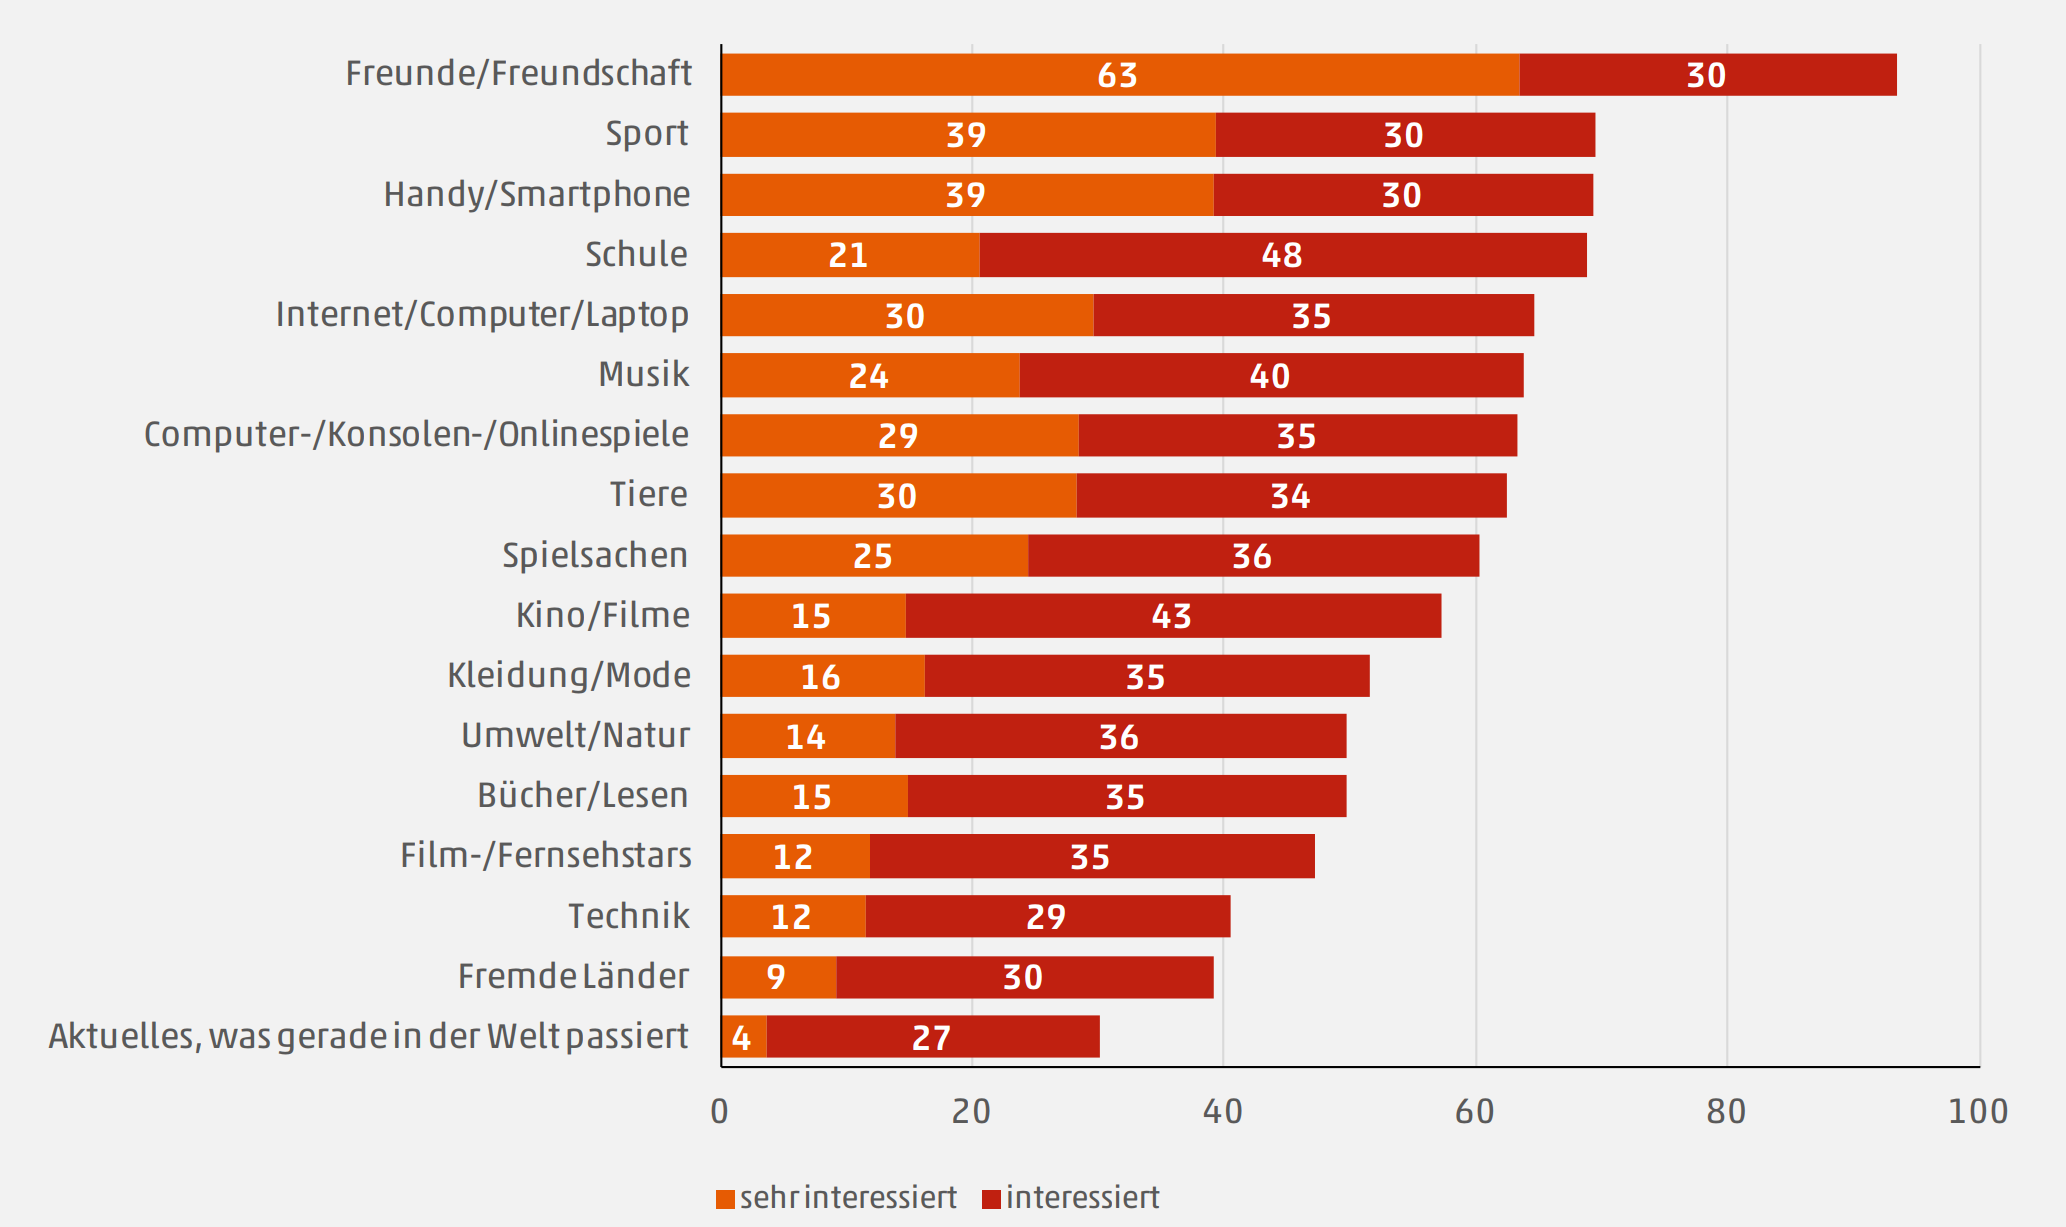
\includegraphics[width=\textwidth]{img/kimstudie.png}
    \caption{Quelle: KIM 2018~\cite{feierabend2018kim}, Angaben in Prozent, Basis: alle Kinder, n=1.231}
    \label{fig:kim_studie}
\end{figure}

\newpage

\section*{Empirische Belege für das Eintreten der behaupteten Wirkungen/en}

Um zu messen, wie gut sich das in dieser Studie gewählte Spiel \textit{(Semideus)} als Lernhilfe eignet wurden abgeleitete Varianten von Fragen vom \textit{Technology Acceptance Model}~\cite{acceptance_of_Information_Technology_1989} verwendet. Es wurde evaluiert, wie die Nützlichkeit empfunden wurde, wie groß die Tendenz es zu benutzen war und wie die Benutzbarkeit empfunden wurde. Für die Beantwortung dieser Fragen wurde eine 6-Punkte \textit{Likert-Skala} verwendet, wobei 1 für ``stimme gar nicht zu'' und 6 für ``stimme voll und ganz zu'' steht.~\cite{Ninaus_Moeller_McMullen_Kiili_2017}

Es wurde auch gemessen, wie qualitativ die Erfahrung für den Benutzer (Schüler/in) des Spiels war. Der Fluss \textit{(experienced flow)}, der während dem Spielen erfahren wurde, wurde direkt nach der letzten Trainingseinheit mit Hilfe einer modifizierten Version einer \textit{``Flow Short''-Skala} ermittelt. Diese funktioniert ähnlich wie die zuvor genannte Skala, nur diesmal konnte von 1 bis 7 bewertet werden.~\cite{Ninaus_Moeller_McMullen_Kiili_2017}

Für die Studie wurde vor und direkt nach dem Einsatz des Lernspiels die genannten Eindrücke des Spiels und Verständnis von- / Interesse an dem betroffenen, mathematischen Themengebiet der Schüler geprüft. Um nun auswerten zu können, ob die Schüler sich im Durchschnitt verbessert haben, wurde ein \textit{t-Test} durchgeführt. \textbf{TODO: VIELLEICHT BESSER BESCHREIBEN} Man konnte erkennen, dass die durchschnittliche Rate mit der die Schüler Aufgaben (die im Spiel trainiert wurden - Zahlenlinien-Abschätzung, Vergleichs- und Ordnungs- Aufgaben) richtig lösen sich potentiell verbessert haben. \\ Vorher (M = 69\%; SE = 13\%), nachher (M = 80\%; SE = 11\%). \textbf{TODO: what's SE}

\newpage

\begin{quote}
    \textit{``As  hypothesized  (Hypothesis  1),  students improved significantly in their rational number knowledge from pre- to posttest [(t(31) = 6.37; p < .001;Cohen's d = 1.13] indicating that our game-based training was effective.''}\hfill~\cite{Ninaus_Moeller_McMullen_Kiili_2017}
\end{quote}

\textbf{... would continue with \ \ Ninaus\_Moeller\_McMullen\_Kiili\_2017 \ \ chapter 3.2}

\newpage

\printbibliography

\end{document}